% !TEX root = main.tex

%%%%%%%%%%%%%%%%%%%%%%%%%%%%%%%%%%%%%%%%%%%%%%%%%%%%%%%%%%%%%%%%%%%%%%%%%%%%%%%%%%%%%%%%%%%%%%%%
\section{実験}
%%%%%%%%%%%%%%%%%%%%%%%%%%%%%%%%%%%%%%%%%%%%%%%%%%%%%%%%%%%%%%%%%%%%%%%%%%%%%%%%%%%%%%%%%%%%%%%%

\subsection{実験器具}
TEKTRONIX TBS1022 オシロスコープ,ソレノイドコイル,磁気プローブ,
ロゴスキーコイル,高電圧パルス大電流発生電源,抵抗$(220\,\si{k\Omega})$,可変抵抗$(<20\,\si{\Omega})$

\subsection{セットアップ}
\begin{enumerate}
    \item 図2のように実験配置を組み立てる.ただし,外部抵抗$R$(可変抵抗)は
    臨界制動波形となる抵抗値になるように調整し,接続する.
\end{enumerate}
\begin{figure}[!ht]
    \centering
    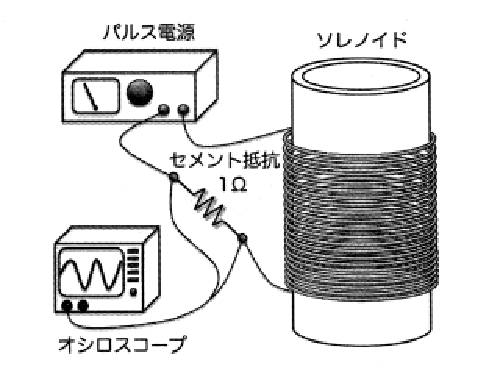
\includegraphics[scale=1]{figure2.pdf}
    \caption{実験装置}
\end{figure}

\newpage

\subsection{-磁気プローブによる磁場測定}
\begin{enumerate}
    \item 磁気プローブのターン数$N$と断面積$S$を実測により求め,記録する.
    \item 図3のように実験器具を配置し,磁気プローブをソレノイド中心軸上の適当な
    位置に保持し,放電する.この際,充電電圧は$50\,\si{\volt}$程度とし,
    その値を記録する.
    \item 抵抗$R$の両端は臨界制動波形$V_R$が現れ,磁気プローブからは出力波形
    $V_{co}$が得られることを確認する.
    \item 磁気プローブをソレノイド中心軸上に沿って動かしながら,ソレノイド
    中心軸上の$z$座標と,その点で得られた臨界制動波形$V_R$および出力波形$V_{co}$
    を記録する.ただし,磁束密度分布$B_z(z)$が滑らかに算出できるように細かく
    測定を行う.
\end{enumerate}
\begin{figure}[!ht]
    \centering
    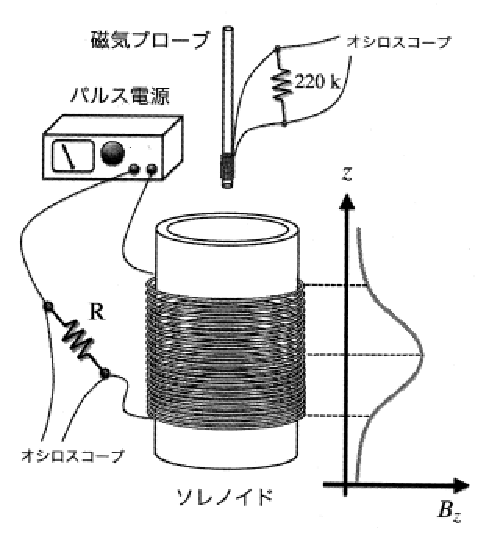
\includegraphics[scale=1]{figure3.pdf}
    \caption{実験課題1における実験配置}
\end{figure}

\newpage

\subsection{ロゴスキーによる電流測定}
\begin{enumerate}
    \item ロゴスキーコイルのターン数$N$,断面積$S$,円周長さ$l$の値を実測
    より求め,記録する.
    \item 図4のように実験器具を配置し,実験を行う.この際,充電電圧値を記録する.
    \item 抵抗$R$の両端は臨界制動波形$V_R$が現れ,ロゴスキーコイルからは
    出力波形$V_e$が得られることを確認する.
    \item ロゴスキーコイルを貫く導線の数(鎖交電流)を徐々に変化させて,
    鎖交数と得られた出力波形を記録する.
\end{enumerate}
\begin{figure}[!ht]
    \centering
    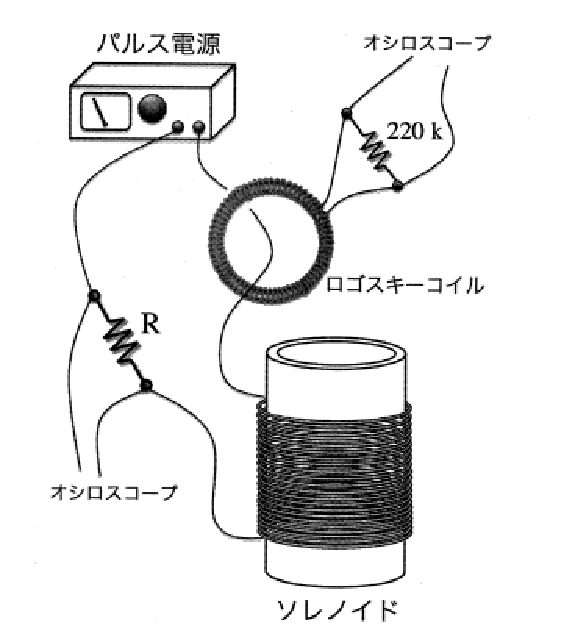
\includegraphics[scale=1]{figure4.pdf}
    \caption{実験課題2における実験配置}
\end{figure}